\documentclass[a4paper,12pt,fleqn]{report}
\linespread{1.3}
\usepackage{color}
\usepackage{graphicx}
\usepackage{natbib}
\usepackage[colorlinks]{hyperref}
\usepackage{url}
\usepackage{amsmath}
\usepackage{amssymb}
\usepackage{array}
\usepackage{verbatimbox}
\usepackage{listings}
\usepackage[ruled,linesnumbered]{algorithm2e}
\usepackage[autostyle]{csquotes}
\setlength{\oddsidemargin}{0.7in}
\setlength{\evensidemargin}{0.7in}
\graphicspath{{images/}}
\author{Jamie Mac Manus}

\hypersetup{
colorlinks=true,
linktoc=all,
linkcolor=black,
citecolor=black,
}

\DeclareRobustCommand{\bbone}{\text{\usefont{U}{bbold}{m}{n}1}}
\DeclareMathOperator{\EX}{\mathbb{E}}% expected value

\definecolor{dkgreen}{rgb}{0,0.6,0}
\definecolor{gray}{rgb}{0.5,0.5,0.5}
\definecolor{mauve}{rgb}{0.58,0,0.82}

\lstdefinestyle{MyFrame}{frame=tb}
\lstdefinestyle{numbers} {numbers=left, stepnumber=1, numberstyle=\tiny, numbersep=10pt}


\lstdefinestyle{Python} {
language=Python,
style=numbers,
style=MyFrame,
frame=none,
backgroundcolor={},
aboveskip=3mm,
belowskip=3mm,
showstringspaces=false,
columns=flexible,
numberstyle=\tiny\color{gray},
keywordstyle=\color{blue},
commentstyle=\color{dkgreen},
stringstyle=\color{mauve},
breaklines=true,
breakatwhitespace=true,
tabsize=3
}

\lstset{language=Python,frame=lines}


\begin{document}
%%
%% Author: jamie
%% 04/10/18

\begin{titlepage}

    \begin{center}

        \vspace*{1.5cm}

        \Huge

        \textbf{Learning to Play no limit Texas Hold'em Using Reinforcement Learning}

        
\includegraphics[width=0.8\textwidth]{ul.jpg}

        \Large
        Department of CSIS

        \vspace{.25cm}
        \textbf{Bachelor of Science in Computer Systems}

        \vspace{.25cm}
        \textbf{Author: } Jamie Mac Manus

        \vspace{.25cm}
        \textbf{ID: } 15147312

        \vspace{.25cm}
        \textbf{Supervisor: } J.J Collins

    \end{center}

\end{titlepage}
%%
%% Author: jamie
%% 04/10/18
%%

\begin{abstract}
    Abstract
\end{abstract}

\newpage
\pagenumbering{Roman}
%%
%% Author: jamie
%% 02/04/19
%%

% Preamble
\section*{Acknowledgements}\label{sec:acknowledgements}

First I would like to thank my FYP supervisor, Mr. J.J Collins for
his constant support, feedback, and guidance on the project.
I came to him with the broad aim of applying reinforcement learning to poker and through
his expertise and engagement he was able to help me find a path for the project that
tread the line of ambition and feasibility.
Throughout the year J.J and I organised weekly meetings in which he provided invaluable
feedback that led the project forward.
I also greatly appreciate his patience as I worked to gain familiarity with a complex
new area of computer science.

I would also like to thank my family for their support,
and to my friends with whom many fun times were had throughout my time in college.

I would like to thank Rory Egan, Dan Noonan and Kevin Moynihan with whom I collaborated on a
number of projects during the four-year course.
Their effort, talent, and insights made project work a painless task throughout the years.

I would like to thank Dr. Jim Buckley for his work as FYP coordinator.

Finally, I would like to thank the CSIS faculty and staff who have all contributed
to a very positive four years of learning in this department.
This is especially the case for all the lectures and TAs that I have had over the
years who helped me develop a foundational CS knowledge that stood me in good stead for this project.
\setcounter{tocdepth}{2}
\setcounter{figure}{49}
\tableofcontents
\listoffigures
%%
%% Author: jamie
%% 05/04/19
%%
\pagebreak

\section*{List of Abbreviations}\label{sec:listOfAbbreviations}

\begin{itemize}
    \item \textbf{ACPC} - Anual Computer Poker Competition
    \item \textbf{BR} - Best Response
    \item \textbf{DP} - Dynamic Programming
    \item \textbf{FP} - Fictitious Play
    \item \textbf{FSP} - Fictitious Self Play
    \item \textbf{GWFSP} - Generalised Weakened Fictitious Self Play
    \item \textbf{MC} - Monte Carlo
    \item \textbf{MCTS} - Monte Carlo Tree Search
    \item \textbf{MDP} - Markov Decision Process
    \item \textbf{ML} - Machine Learning
    \item \textbf{NFSP} - Neural Fictitious Self-Play
    \item \textbf{POMDP} - Partially Observable Markov Decision Process
    \item \textbf{RL} - Reinfocement learning
    \item \textbf{TD} - Temporal Difference
    \item \textbf{UCB} - Upper Confidence Bounds
    \item \textbf{UCT} - Upper Confidence Bounds Applied to Trees
\end{itemize}
\clearpage

\pagenumbering{arabic}
\chapter{Introduction (10)}
\label{ch:intro}
In this section I will introduce the subject area of this Final year Project (FYP).
I will then go on to give an overview of the report, establish some goals for the project along with some of
the motivations for choosing this subject area.


\section{Overview (3) w5}\label{sec:overview}
Since the inception of machine learning, games have been a key problem area that has seen a lot of focus from
top academics.
Furthermore, the development of some machine learning strategies that can be applied to games has also lead to these
strategies being applied in many different domains, many of which being very beneficial in practice.


\section{Objectives (2) w4}\label{sec:objectives}
\subsection{Reinforcement Learning and Leduc Hold'em}\label{subsec:primaryObjectives}
In the past, methods such as counterfactual regret minimization (CFR) have been used to develop agents that can
play no-limit texas hold'em to a superhuman level.
This includes the 2018 champion of the Annual Computer Poker Competition, slumbot\cite{jackson2013slumbot}.
There have also been attempts to solve the limit version of the game using reinforcement learning
(RL)\cite{heinrich2016deep}.

Throughout the course of this project I will be using an iterative approach to solving the problem.
As such the first agent that I will develop will seek to tackle a simplified version of hold'em.
Specifically I will be attempting utilise the algorithm outlined in\cite{heinrich2015fictitious} to develop an agent
that can play a simplified version of texas Hold'em called Leduc Hold'em.

\subsection{Apply the Algorithm to a More Complex Poker Variant}\label{subsec:pokerPlayingAgent}
When I have successfully applied the algorithm to Leduc Hold'em my goal is to then apply the same algorithm
to a more complex game.

\subsection{Web Interface For to Play Against the Agent}\label{subsec:webInterface}
The focus of this report will largely be research.
However it is also my goal to create a product that will be fun and useful for the general public.
As such another objective will be to create a website that will allow users to play heads-up against the final product.

\subsection{Understanding Reinforcement Learning}\label{subsec:understandingRL}
As this project is very specific and academic, one of the larger challenges will be to gain a strong knowledge
of the domain.
This means learning the history of RL, the types of problems that it has been used to solve and the specific details of
different RL algorithms.

\subsection{Understanding AI and Imperfect Information Games}\label{subsec:aiInImperfectinfo}
A successful project will require a high degree of knowledge from the broader domain of RL. However, it is also the case
that I must become closely familiar with the existing academic literature in the area of RL with respect to imperfect
information games.
This will allow me to avoid taking approaches that have previously shown to fail and also allow me to contribute to
the existing literature without simply replicating what has already been done.


\section{Contribution (1) w5}\label{sec:contribution}

\section{Methodology}\label{sec:methodology}


\section{Motivation (2) w5}\label{sec:Motivation}
\chapter{Background (18)}
\label{ch:background}

The aim of this chapter is to give the reader background information on the problem domain in order for them
to understand the rest of the report.
Then we will go into more detail on the areas of reinforcement learning, game theory and texas hold'em.
However, this final year project is heavily based on machine learning so I think it is important for the reader to have
some background on this area first.

Machine learning is an area of computer science that tackles how we construct computer programs that improve
with experience\citep{mitchell1997machine}.
The term was coined by Arthur Samuel in his 1959 paper where he discussed machine learning methods using
checkers.
Since then there has been a great deal of advancement in the field.
Some of the notable early contributions being the discovery of recurrent neural networks in 1982 and
the advancement of reinforcement learning by the introduction of Q-Learning in 1989.
Recently we have seen some of this early academic work culminate in more practical achievements such as
Facebook's DeepFace system which, in 2014,  was shown to be able to recognise faces at a rate of 97.35\% accuracy,
a rate that is comparable to that of humans.
Another example of recent achievement is Google's AlphaGo program which, in 2016, became the first program to beat
a professional human player.

It should be becoming clear that machine learning can be a solution to a wide scope of problems and as
both hardware and software continue to improve this scope will only continue to widen.
We are starting to see machine learning systems become a key component of many companies business model.
Since certain machine learning techniques are great at prediction, machine learning has been widely used
for content discovery by companies such as Google and Pinterest.
Other business applications include the use of chatbots as a part of customer service, self-driving cars
and even in the field of medical diagnostics.


\section{Reinforcement Learning}\label{sec:reinforcementLearning}
When I began to research the possibility of creating a texas hold'em playing agent using machine learning techniques it
quickly became apparent that reinforcement learning would be the most suitable approach.
Thus I began to research the area in order to gain an in-depth understanding of the area.
This research included a Udemy course as well as reading in part Reinforcement Learning: An Introduction
a book published in 1998 by Andrew Barto and Richard S. Sutton.
In the following section I will outline the findings rendered by this research.

\begin{figure}[ht]
    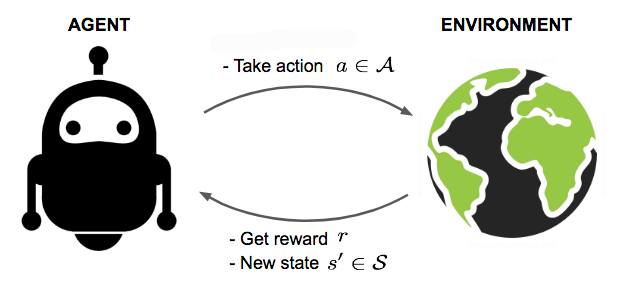
\includegraphics[scale=.5]{RL_illustration.png}
    \caption{Reinforcement Learning}
\end{figure}

Reinforcement learning is a way of programming agents by reward and punishment without needing to specify how the
task is to be achieved\citep{kaelbling1996reinforcement}.
As such the primary components of a reinforcement learning problem are an agent which exists in an environment.
From a simplified perspective we can think of the environment as a set of states, actions and rewards.
The objective for the agent is to maximise cumulative reward.
This is done by developing a policy that will dictate which actions should be taken in each state.

\subsection{Explore-Exploit Dilemma}\label{subsec:exploreExploit}
When it comes to reinforcement learning one of the first questions that we have to ask is how we explore
the state space.
An example that is often used to conceptualize this problem is the multi armed bandit problem.
Let's say an agent is in a room with a number of gambling machines.
Each of these machines has an arm that, when pulled will return a reward of 0 or 1 based on some underlying
probability\citep{kaelbling1996reinforcement}.
The agent has a limited number of total pulls.
So the question becomes how do we distributed these pulls in order to maximise return?
Well, first we have to ensure that we explore enough that we find the machine with the best reward probability
and second, we must then exploit this machine to the best of our abilities.

\begin{figure}[ht]
    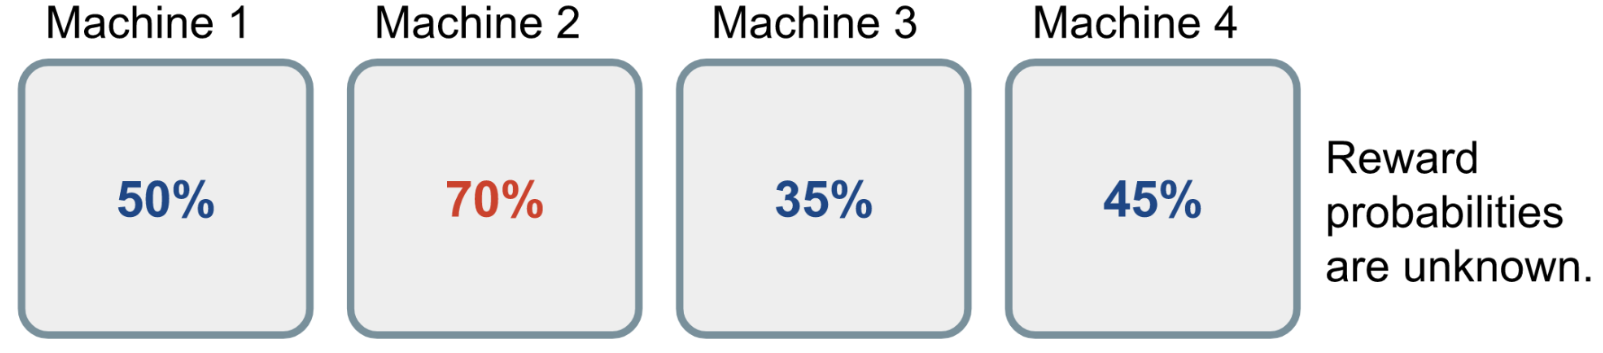
\includegraphics[scale=.25]{bandit.png}
    \caption{Multi Armed Bandit}
\end{figure}

There are a number of approaches that can be taken to solve this problem, we will now briefly discuss two of these
methods.

\subsubsection{$\epsilon$-Greedy Solutions}\label{subsec:eGreedy}
The first approach that we will discuss is the $\epsilon$-greedy strategy.
This approach was first proposed by Watkins\citep{watkins1989learning} and is a very simple and widely used method.
The $\epsilon$-greedy strategy involves choosing a random lever some proportion $\epsilon$ of the time, and
choosing the lever that has been established to give the highest reward the rest of the time.

There are a number of variations of this method, the first being the $\epsilon$-first strategy.
With this strategy we take all of our random choices first, allowing us to establish the best bandit,
after which we exploit this bandit.
However, as stated in\citep{vermorel2005multi} this simple approach is sub-optimal because asymptotically,
the constant factor prevents the strategy from getting arbitrarily close to
the optimal lever.

This is where the $\epsilon$-decreasing strategy becomes useful.
Here, the proportion of random lever pulls decreases with time.
Generally if our initial epsilon value is $\epsilon_0$ then our epsilon value at time $t$ will be
$\epsilon_t = \frac{\epsilon_0}{t}$.

\subsubsection{Interval Estimation Strategy}
Another approach that can be used is called the interval estimation strategy.
With this method we initially give an optimistic estimate of the reward to each bandit within a certain
confidence interval.
Then we simply take a greedy approach to our exploration.
Less explored bandits will have a artificially higher reward estimate and thus they will be greedily chosen,
thus allowing us to evaluate each of the bandits.

In the context of reinforcement learning, state space exploration through the $\epsilon$-greedy approach is
generally sufficient.

\subsection{Markov Decision Processes}\label{subsec:mdp}
Reinforcement learning problems are generally modelled according to what is called a markov decision process.

\begin{itemize}
    \item S - a set of states.
    \item A - a set of actions.
    \item P - a set of state transition probabilities
    \item R - a set of rewards
    \item $\gamma$ - a discount factor
\end{itemize}

\subsection{Policy Evaluation and Policy Improvement}\label{subsec:policyEvalPolicyImp}
As mentioned above the primary focus of reinforcement learning is to find a policy (denoted by $\pi$) that allows
the agent to take actions in states that lead to the maximum possible reward.
There are two primary problems that we must solve in order to do so.

The first is called the prediction problem, also known as policy evaluation.
This involves computing the values of states given some arbitrary policy\citep{sutton1998reinforcement}.
For example a state would have a high value if the reward for reaching that state was high.
A state would also have a high value if we were only one action away, according to the supplied policy,
from a state that renders a high reward.
However a state would have a low value if, according to the policy, there was no path to a state that
would return a positive reward in the foreseeable future.

The second problem is known as the control problem, also known as policy improvement.
This involves changing the policy in order to improve our cumulative reward.
The policy improvement process can only occur when the we have performed policy evaluation.
Let's say, after our evaluation step, we know the value of some state $s$.
Note that this value is calculated with the condition that we take some action $a$ in state $s$.
But, if we take some other action $a'$ would this render a higher value for $s$?
If the answer is yes then we update the policy.

These two operations can be seen as the core of reinforcement learning.
In the next section we will discuss different reinforcement learning methodologies.
Some of the main differences are in how method each approaches the prediction and control problems.

\subsection{Dynamic Programming (3)}\label{subsec:dp}
Dynamic programming (DP) refers to a collection of algorithms that can be used to compute optimal policies given a
perfect model of the environment as a Markov decision process\citep{sutton1998reinforcement}.
Dynamic programming provides a basis for many algorithms that are used in practical reinforcement learning applications.
An example of such an algorithm is value iteration.
This is where we alternate between policy evaluation and policy improvement in order to converge towards an optimal
policy.

\subsection{Monte Carlo (3)}\label{subsec:mc}
In Monte Carlo, unlike dynamic programming, we do not assume complete knowledge of the environment.
Monte Carlo methods require only experience-sample sequences of states, actions, and rewards from interaction with
an environment\citep{sutton1998reinforcement}.
Monte carlo evaluation is an episodic process this means that we only update our action values after an episode
has completed.
%Policy evaluation: simply average many returns that start in the state.
%Policy improvement: estimate action values in order to avoid reliance on state transition dynamics.
%(simply choose the best action for the policy in a given state)


\subsection{Temporal Difference Learning (3)}\label{subsec:td}


\section{Supervised Learning}\label{sec:supervisedLearning}
Supervised learning involves an agent which observes some example input-output pairs and learns
a function that maps from input to output.\citep{russell2016artificial}.
This learned function can then be used on new input data, that wasn't used to train the agent and the
agent should be able to give an accurate output.
As such this learning task is a generalization problem.
The agent must be able to identify general features of the input data and how they map to the output.
Common examples of

\section{Game Theory}\label{sec:gameTheory}

\section{Texas Hold'em}\label{sec:thIntro}
Texas hold'em is one variant of the family of games called poker.
Poker is a group of card games that combine gambling, strategy and skill.
All poker variants have three core similarities.
There is betting involved, there is imperfect information (ie cards remain hidden until the end of a hand)
and the winner is determined by combinations of cards.
We will now discuss texas hold'em poker in more detail.

\subsection{Game Structure}\label{subsec:bettingRounds}
Texas hold'em consists of four betting rounds.
Initially each player is dealt two private cards.
These remain face down and only the person who received these cards may view them.
In the next three rounds five public cards are dealt face up on the table.
The second round of dealing is called the flop, where three cards are dealt.
The third round is called the turn where one additional public card is dealt.
Finally in the fourth round another card is dealt which is called the river.

At each round, after the cards are dealt, the players are given the opportunity to take a number of betting
related actions.
We will discuss the permitted actions in the next section.

In order for players to be incentivized to continue playing in a wider array of situations, blinds are required.
Blinds are a mandatory bet that must be posted by two of the players present at the game.
These two bets are called the big blind and the small blind, the big blind being twice that of the small blind.
As hands are played the big and small blinds are posted by different players in order to distribute the cost fairly.

The big and small blind are the first two bets that contribute to what's called the pot.
The pot is the collection of all of the current chips bet by the players.
When a player wins a hand then what they receive in return is the pot.

The final structural component of the game is player stacks.
Each player will start the game with a certain amount of chips.
If a player wins a pot then all of the chips in the pot are transferred to the winners stack.

\subsection{Actions}\label{subsec:actions}

\subsection{Hand Values}\label{subsec:handValues}


%%
%% Author: jamie
%% 05/10/18
%%
\chapter{Application Development (10)}\label{ch:development}

\section{Requirements}\label{sec:requirements}
\section{Design}\label{sec:design}
\section{Backend API}\label{sec:api}
\section{Frontend Website}\label{sec:website}
\section{Testing}\label{sec:testing}
\section{Issues}\label{sec:issues}

%%
%% Author: jamie
%% 04/10/18
%%

% Document
\chapter{Empirical Studies}\label{ch:empirical}

\section{Overview}\label{sec:empOverview}
In this chapter, we will cover a number of experiments that were conducted in order to investigate
the performance of the different algorithms implemented in order to tackle Leduc Hold'em.
We will begin with a simplified version of MCTS for POMDPs and will incrementally add to this
method in order to see how the performance of our agent evolves.
In the table below we have listed the template that we will follow when conduction these experiments.


\addvbuffer[12pt 0pt]{\begin{tabular}[ht]{ | p{2cm} | p{10cm} | }
    \hline
    \textbf{Section} & \textbf{Rationale} \\
    \hline
    Objective & This section will contain an explanation of the purpose of the experiment along with
    how it was carried out \\
    \hline
    Experimental Parameters & This section outlines how we parameterised the experiment. \\
    \hline
    Results & This section will detail the results acquired from the experiments conducted \\
    \hline
    Analysis & In this section we will examine our results and try to provide insight into the
    reasoning behind these results \\
    \hline
\end{tabular}}

\section{Experiment 1 - UCT Versus Random Player}\label{sec:expmeriment1}
The first experiment conducted involved a simplified version of the algorithm outlined in\citep{heinrich2017reinforcement}.
We set an initial goal of using a random player as our benchmark opponent in order to demonstrate how
this algorithm could exploit such a player's strategic inefficiencies.

\subsection{Objective}\label{subsec:objective1}
The goal of this experiment is to implement UCT for Leduc Hold'em.
The UCT agent will play against a random player and learn a strategy to exploit this player for
maximal reward.
Although we are interested in the results gained from playing against the random player we treat the
outcome of this experiment as a baseline for our subsequent results.
The reasoning for this is that the difficulty in finding a winning strategy against a random player
is not high.
In fact, at each point in the game that the random player can take an action it is
just as likely to fold it's cards, regardless of their value, as it is to take any other action.
This means that for our agent the intelligent strategy is to merely retain all but the
very worst of its hands.
Thus we can think of the strategy learned by this initial agent as a broad
categorisation between very weak hands and all other hands.
Thus we expect that the exploitability of the resultant agent will be relatively high.
Our agent will not have learned all of the strategic intricacies of the game
and it will not react strategically to the opponent's play.
Rather, it will simply know how to beat a 'dumb' random player.
This will give us a platform to build a more sophisticated agent through different mechanisms such as
self-play in the subsequent experiments.

\subsection{Experimental Parameters}\label{subsec:algAndCoding1}
For each experiment, we will list the parameters that were used to instantiate the agent.
These parameters either refer to the execution time of the algorithm or are a part of
the group of parameters that were outlined in Algorithms 1, 2 and 3.
In the case of each experiment, we replicate the values outlined in\citep{heinrich2017reinforcement}.
If there is a deviation from these values the reasoning behind it will be explained.

Below are listed the key parameters for the first experiment:
\begin{itemize}
    \item \textbf{Iterations} - 500,000
    \item \textbf{Repetitions} - 20
    \item \textbf{$c$ - exploration constant} - 18
\end{itemize}

\subsection{Results}\label{subsec:results1}
The first metric that was used in order to analyse the results of this experiment is cumulative reward.
This is simply the sum of the output of the reward function over time.
This function directly corresponds to the size of the pot won or lost in the game,
thus the reward can be either positive or negative.
In figure 4.1 we see the reward over time increasing.
In order to obtain these results, the algorithm was run for 10,000 iterations and this process was repeated 100 times.
Our cumulative rewards were then averaged at each iteration across these 100 repetitions to give the graph shown.
Figure 4.2 shows the rate of increase in cumulative reward or the average reward over time.
In the case of figure 4.2, we applied the UCT algorithm for 500,000 iterations and
repeated this process 20 times, averaging the results.

\begin{figure}[ht]
    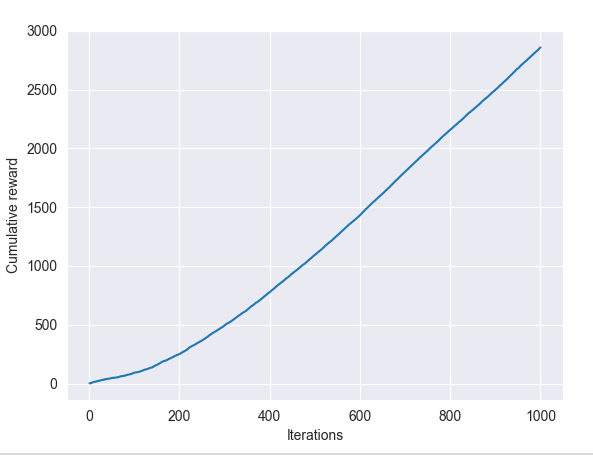
\includegraphics[scale=.8]{images/cumulative_reward_mcts_vs_random.png}
    \caption{UCT cumulative reward vs random player - 10000 Iterations}
\end{figure}

\begin{figure}[ht]
    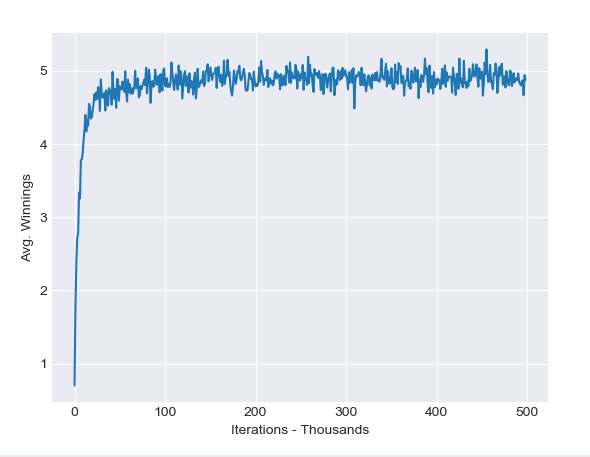
\includegraphics[scale=.7]{images/avg_reward_500000__20_random.png}
    \caption{UCT average reward vs random player - 500000 Iterations}
\end{figure}

The second metric used to produce results was exploitability.
This is a measure of the reward that can be gained by playing a best response strategy
against the agent.
In figure 4.3 we see that the exploitability of our agent is quite high throughout, with an
initial dip followed by a divergence towards 4.9.

\begin{figure}[ht]
    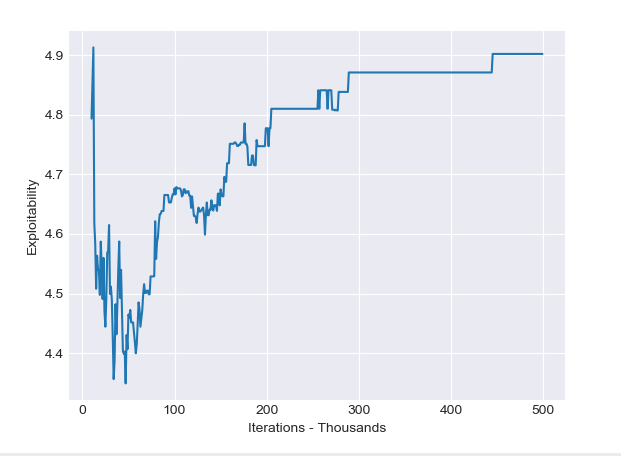
\includegraphics[scale=.7]{images/exploitability_500000_20_random.png}
    \caption{UCT exploitability vs random player - 500000 Iterations}
\end{figure}

\subsection{Analysis}\label{subsec:analysis1}
We will first analyse our results from the cumulative reward metric.
As shown by figure 4.1 we see that initially there is a gradual increase in cumulative reward,
with the slope growing until there is a constant rate of increase.
This demonstrates that during the initial phase of the algorithm we have not yet uncovered
the most beneficial action selection for all states and the exploration phase is still in effect.
However, by visual inspection, we can see that over time the rate of increase in cumulative
reward begins to stabilise which indicates that a concrete strategy that can exploit
the random play has been established.
This hypothesis is further supported by figure 4.2 as we see a dramatic upswing
in the rate of increase of cumulative reward followed by a leveling of the graph.

As mentioned the exploitability value throughout this figure 4.3 is relatively poor with an initial dip followed
by a divergence.
This is most likely explained by the fact that we are not playing against a rational player.
As such our strategy is strong when it comes to maximally exploiting an irrational, random player
but if we then substitute this irrational player for a rational player, the results will not be favourable.

\section{Experiment 2 - UCT Self-Play} \label{sec:experiment2}
In our second experiment, the agent was trained against itself.
In other words, two instances of the agent were generated and allowed to develop strategies
through self-play.

\subsection{Objective}\label{subsec:objective2}
The objective of this experiment was to implement Heinrich's extensive form MCTS using UCB action
selection (ie extensive form UCT).
Here a significant improvement in the exploitability of the agent was expected.
This was due to the fact that the opposing agent is rational, in that it learns
through experience.


\subsection{Experimental Parameters}\label{subsec:algAndCoding2}
Below are listed the key parameters of the experiment
\begin{itemize}
    \item \textbf{Iterations} - 500,000
    \item \textbf{Repetitions} - 10
    \item \textbf{$c$ - exploration constant} - 18
\end{itemize}

\subsection{Results}\label{subsec:results2}
In the case of self-play both agents develop intelligent strategies.
This means that we do not see any significant trends in cumulative reward or average reward over time
due to the fact that neither player has an advantage.
This is shown in figure 4.4.
\begin{figure}[ht]
    \includegraphics[scale=.7]{images/avg_winnings_self-play.png}
    \caption{UCT average reward over time - self-play - 500000 Iterations}
\end{figure}
As such these metrics were disregarded and exploitability became the sole metric.
Once again we applied the algorithm for 500,000 iterations, repeating this process 10 times
and averaging the results.

In figure 4.5 it can be seen that there is a notable improvement in exploitability, with lows of 3.5 initially
but over time the values begin to diverge once again back towards 4.6.

\begin{figure}[ht]
    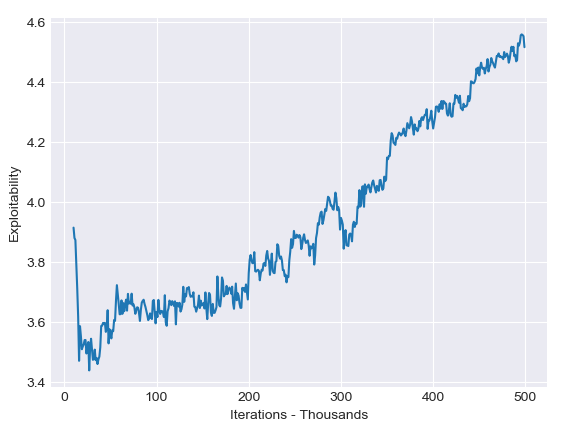
\includegraphics[scale=.7]{images/exploitability_self-play_deterministic_500000.png}
    \caption{UCT exploitability - self play - 500000 Iterations}
\end{figure}

\subsection{Analysis}\label{subsec:analysis2}
The results gleaned from this experiment were unexpected to a degree.
Heinrich had shown exploitability reaching lows of .8 and diverging to 1.5 in a similar experiment.
Although a similar trend was shown here our exploitability values were significantly higher.
This could potentially be explained by differences in the algorithm used to calculate exploitability
or the implementation of UCT itself.

On further inspection of the search trees generated, along with the best response tree (see chapter 3)
there appeared to be an over-fitting to the opponent's strategy over time.
Notably, both instances of the agent were playing more conservatively than expected.
This meant that the best-response player could regularly force our agent to fold in
situations where folding against a less conservative player would be illogical.
In order to conceptualize this phenomenon, the following example is given.
Let's say player one is very conservative and they decide to only raise in the second round of the game when they
have a pair of aces.
This means that over time player two will only receive highly negative rewards for the states in
which player one has raised in the second round.
In fact, in this case, it is more beneficial for player two to simply fold if player one raises in
the second round of the game.
When a new player is introduced to the system, however, they can take advantage of this
behavior by simply raising more frequently in the second round of the game.
This type of strategic feedback loop is characteristic of deterministic strategies due to the
fact that breaking such a loop becomes less and less likely the closer we get to purely greedy action selection.


\section{Experiment 3 - Smooth UCT}\label{sec:experiment3}
The final experiment conducted during our empirical studies utilised both self-play
and average strategy sampling.
Ie smooth UCT was used.

\subsection{Objective}\label{subsec:objective3}
The objective of this experiment was to implement Smooth UCT as outlined in\citep{heinrich2017reinforcement}.
Again a significant improvement in exploitability was expected at this stage due to the fact
that stochastic strategies were now in use in the training phase.
Heinrich showed smooth UCT to converge to an approximate Nash's equilibrium for Leduc Hold'em.
As such the primary goal for this experiment is to replicate these results as closely as possible.
This goal was set with the caveat that, as mentioned in section 3.2.2 only deterministic strategies
could be evaluated for exploitability at this stage of development.
As such the exploitability values produced may be higher than expected.

\subsection{Experimental Parameters}\label{subsec:algAndCoding3}
Note that in the case of smooth UCT the $d$ parameter has been modified, with Heinrich's
original value being .002.
It was found through experimentation that Heinrich's stated value did not provide a significant
improvement compared to experiment 2's results.
However, when increased to .1 we saw our best exploitability results.

Below are listed the key parameters of the experiment:
\begin{itemize}
    \item \textbf{Iterations} - 1,000,000
    \item \textbf{Repetitions} - 10
    \item \textbf{$c$ - exploration constant} - 18
    \item \textbf{$\gamma$} - .01
    \item \textbf{$\eta_0$} - .9
    \item \textbf{$d$} - .1
\end{itemize}

\subsection{Results}\label{subsec:results3}
For this experiment exploitability was once again the sole metric used.
In this case, the algorithm was run for 1,000,000 iterations and 10 repetitions with the results averaged.
The results of the experiment are shown in figure 4.6.
\begin{figure}[!ht]
    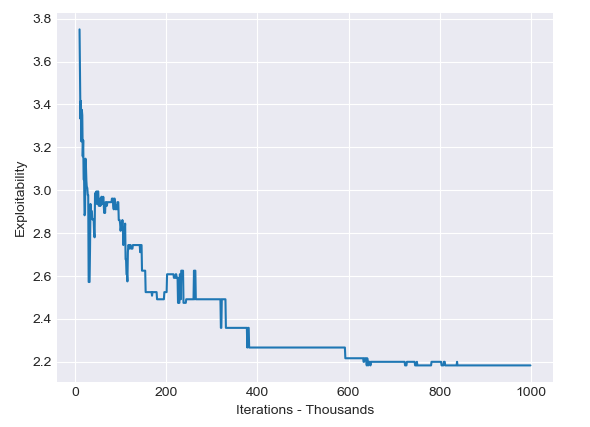
\includegraphics[scale=.7]{images/exploitability_self-play_stochastic_1000000.png}
    \caption{Smooth UCT exploitability - self play - 1000000 Iterations}
\end{figure}

Here we see a significant improvement compared to the last experiment in which deterministic strategies were used.
There is no longer a tendency for exploitability to diverge as there it had in experiment 2 with
early exploitability values of 3.8 converging towards 2.2 and stabilising.
However, these values are still less favourable than those demonstrated by Heinrich who achieved
exploitability of roughly .5 after 1,000,000 iterations.

\subsection{Analysis}\label{subsec:analysis3}
The relative success of this experiment compared to the others demonstrates the value of
utilising stochastic strategies in these scenarios.
The over-fitting effect mentioned in experiment 2 was no longer an issue.
This is likely due to the fact that when the average strategy is being sampled there is a
chance to break out of such a feedback loop as all possible actions will be sampled over time.

Although Heinrich's benchmark was not met, there are a number of extenuating factors that must be
considered in order to contextualize these results.
Firstly, the starting exploitability value is significantly higher than Heinrich's (3.8 vs 2).
This may indicate that the general methodology for exploitability computation differed across these
two implementations.
Second, due to the scope of the project extensive parameter tuning was not possible.
It's most likely that these results could be significantly improved if the optimal parameter
combination was found for this implementation.
Third, as mentioned, only exploitability calculation for deterministic strategies was performed.
If this had been implemented for stochastic strategies then the exploitability values would
likely have been lower due to the fact that stochastic strategies fare far more favourably in
imperfect information games\citep{heinrich2016deep}.
Finally, the computational resources available for this project were limited and as we could not
fully replicate Heinrich's experiments.
It would have taken a number of days to complete 500,000,000 iterations of the algorithm on the
available hardware.
\chapter{Conclusions}

\section{Summary}

\section{Reflections}

\section{Future Work}


\bibliographystyle{agsm}
\bibliography{references}

\end{document}

